\section{ Bayesian Filter for Tracking Moo-Deng's Behavior I (32)}

\begin{figure}[H]
    \centering
    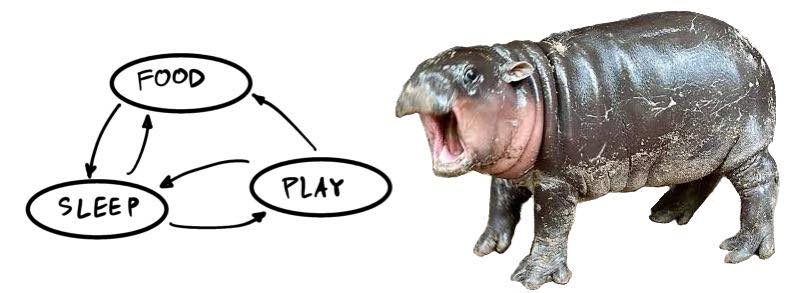
\includegraphics[width=0.65\textwidth]{img/moodeng.jpg}
    \caption{An abstract version of Moo-Deng's enclosure}
    \label{fig:p3c1}
\end{figure}

Khao Kheow Open Zoo in Thailand has gained popularity thanks to its star resident, Moo-Deng, a playful yet feisty Pygmy hippo. To better understand Moo-Deng's daily routine, the zoo has hired a wildlife researcher to track her movements between three key zones: Feeding Area ($A=1$), Resting Area ($A=2$),Playground Area ($A=3$).
Let $\mathbf{x}$ be a vector of probability of Moo-Deng being in the feeding area, the resting area, and the playground area respectively, which can be formally expressed as follows:
\begin{equation*}
    \mathbf{x}=\begin{bmatrix}
    p(A=1) \\ p(A=2) \\ 
    p(A=3)   
    \end{bmatrix}
\end{equation*}
It can be assumed that Moo-Deng only stays in one of these 3 places. Therefore:
\begin{equation*}
\sum_{i=1}^3p(A=i)=\mathbf{1}^\top\mathbf{x}=1
\end{equation*}
After careful observation, the researcher has identified Moo-Deng's behavior patterns:
\begin{itemize}
    \item When Moo-Deng is in the Feeding Area ($A=1$), she has a 60\% chance of staying there, and  a 40\% chance of moving to the Resting Area ($A=2$).
    \item If Moo-Deng is in the Resting Area ($A=2$), she has a 40\% chance of staying there, a 20\% chance of returning to the Feeding Area ($A=1$), and a 40\% chance of moving to the Playground Area ($A=3$).
    \item If Moo-Deng is in the Playground Area ($A=3$), she has a 70\% chance of staying there, a 20\% chance of moving to the Feeding Area ($A=1$), and a 10\% chance of moving to the Resting Area ($A=2$).
\end{itemize}
The behavior of Moo-Deng can be modelled as a transition matrix $\mathbf{A}\in\mathbb{R}^{3\times3}$ such that the following is true:
\begin{equation*}  \mathbf{x}_{k+1}=\mathbf{A}\mathbf{x}_{k}
\end{equation*}
where $\mathbf{x}_k$ denotes the probability vector at the $k^\text{th}$ observation.

Furthermore, the researcher uses a digital sensor system to track Moo-Deng’s location, but the sensor is not perfectly accurate:
\begin{itemize}
    \item When Moo-Deng is in the Feeding Area, the sensor reports Feeding Area with an 80\% accuracy, but it incorrectly reports Resting Area 10\% of the time and Playground Area 10\% of the time.
    \item When Moo-Deng is in the Resting Area, the sensor reports Resting Area 70\% of the time, but it incorrectly reports Feeding Area 20\% of the time and Playground Area 10\% of the time.
    \item When Moo-Deng is in the Playground Area, the sensor reports Playground Area with an 85\% accuracy, but it incorrectly reports Resting Area 10\% of the time and Feeding Area 5\% of the time.
\end{itemize}
At the $k^\text{th}$ observation, the reading from the sensor system can be encoded to a vector of digital values $\mathbf{y}_k$ so that:
\begin{equation*}
    \mathbf{y}_k=\begin{cases}
        \begin{bmatrix}
            1 & 0 & 0
        \end{bmatrix}^\top & \text{if} \quad\text{the measurement displays \texttt{Feeding Area}}\\
        \begin{bmatrix}
            0 & 1 & 0
        \end{bmatrix}^\top & \text{if} \quad\text{the measurement displays \texttt{Resting Area}}\\
        \begin{bmatrix}
            0 & 0 & 1
        \end{bmatrix}^\top & \text{if} \quad\text{the measurement displays \texttt{Playground Area}}
    \end{cases}    
\end{equation*}
Then, the probaiblity of sensor displaying each area can be modelled as follows:

\begin{equation*}
    \begin{bmatrix}
        p(\mathbf{y}_k=\begin{bmatrix}
            1 & 0 &0
        \end{bmatrix}^\top)\\
        p(\mathbf{y}_k=\begin{bmatrix}
            0 & 1 &0
        \end{bmatrix}^\top)\\
        p(\mathbf{y}_k=\begin{bmatrix}
            0 & 0 &1
        \end{bmatrix}^\top)
    \end{bmatrix}=\mathbf{C}\mathbf{x}_k
\end{equation*}
where $\mathbf{C}\in\mathbb{R}^{3\times3}$ is yet to be determined.

\begin{enumerate}[a)]
    \item Assume that Moo-Deng starts in the Feeding Area ($A_0=1$). What is the probability that her subsequent movements will follow the sequence ($2$,$3$,$3$,$1$) in this exact order? Explain your calculation. [4 pts]
    \item Determine the numerical value of the transition matrix $\mathbf{A}$. You must explain your rationale. [5 pts]
    \item Analytically compute the stationary probabilities of Moo-Deng’s location $\mathbf{x}^*$. These are the probabilities that, after many transitions, Moo-Deng will be found in each of the zones regardless of the initial location. You must show your work. [Hint: $??=\mathbf{A}\mathbf{x}^*$] [8 pts]
    
\item Determine the numerical value of the  matrix $\mathbf{C}$. You must explain your rationale. [5 pts]
    
    \item Derive a state estimator based on a Bayesian Filter that estimates the states and probability of Moo-Deng's  based on prior belief $\mathbf{x}_{k-1}$ and the current sensor measurement $\mathbf{y}_k$. You may leave your answer in terms of $\mathbf{A}$ and $\mathbf{C}$. You may also substitute their numeric values. [10 pts]
\end{enumerate}
